\newcommand{\waitingtime}{
\begin{tikzpicture}[
  yscale = 0.8,
  normal/.style={ fill=black!30},
  resource/.style={ fill=black!80},
  waiting/.style={fill=white},
  busywait/.style={fill=black!10, postaction={pattern=north east lines, very thin}},
  release/.style={-latex},
  request/.style={-o},
  complet/.style={-|},
  important/.style={color=red,thick,|-|},
  every text node part/.style={align=center}
]
%general params
\def\th{.4} %task height
\def\tyDown{0} %task a asse y
\def\tyUp{1}
\def\blockdim{(.4,.4)}
\def\arrowdim{(0,.5)}
\def\arrowdimB{(0,.4)}
\coordinate (legend) at (-0.5,2.3);

\begin{scope}

\path(-1.4, 2)node[below]{\textcolor{red}{(1)}};
\path(3.7, 2)node[below] {\textcolor{red}{(2)}};

%tasklines
\draw[very thin, gray] (-.7,\tyDown)node[above,left,black]{$P_2$} -- +(3.2,0);
\draw[very thin, gray] (-.7,\tyUp)node[above,left,black]{$P_1$} -- +(3.2,0);

%axes
\draw[thick, black, -] (-.5,-0.7) -- (-.5, 1.8);
\draw[thick, black, ->] (-1,-.5) -- (2.7, -.5);
% \foreach \x in {0,...,2}\draw[thin, black] (\x, -.6) -- (\x, -.4);

%Processor 1 ==> \tyUp

\draw[release] (0,\tyUp) -- +(0,.8);
\draw[normal]   (0, \tyUp) rectangle +(0.4, \th) node[midway] {{\footnotesize $J_1$}};
\draw[request] (0.4,\tyUp) -- +(0,.8);
\draw[resource] (0.4, \tyUp) rectangle +(0.5, \th) node[color=white,midway] {{\footnotesize  $J_1$}};
\draw[release] (0.9,\tyUp) -- +(0,.8)node[above] {{\tiny $J_3$}};
\draw[normal]   (0.9, \tyUp) rectangle +(0.6, \th) node[midway] {{\footnotesize $J_3$}};
\draw[complet] (1.5,\tyUp) -- +(0, .7);
\draw[resource] (1.5, \tyUp) rectangle +(0.4, \th) node[color=white,midway] {{\footnotesize  $J_1$}};
\draw[complet] (1.9,\tyUp) -- +(0, .7);

%Processor 2 ==> \tyDown

\draw[release] (0.2,\tyDown) -- +(0,.8);
\draw[normal]   (0.2, \tyDown) rectangle +(0.6, \th) node[midway] {{\footnotesize $J_2$}};
\draw[request] (0.8,\tyDown) -- +(0,.8);

\path(0.8, -.6)node[below]{{\tiny $t_1$}};
\draw[thin, black] (0.8, -.6) -- (0.8, -.4);

\path(1.9, -.6)node[below]{{\tiny $t_2$}};
\draw[thin, black] (1.9, -.6) -- (1.9, -.4);

\draw[important] (0.82,\tyDown + 0.25) -- +(1.06,0) node[midway,yshift=0.2cm]{\scriptsize \textcolor{blue}{(a)}};

\draw[resource] (1.9, \tyDown) rectangle +(0.6, \th) node[color=white,midway] {{\footnotesize  $J_2$}};
\draw[complet] (2.5,\tyDown) -- +(0, .7);

\path(0, -1)node[xshift=1cm,below]{{\footnotesize \textcolor{blue}{(a)} queueing time}};

\end{scope}

\begin{scope}[xshift=4.8cm]

%tasklines
\draw[very thin, gray] (-.7,\tyDown) -- +(3.2,0);
\draw[very thin, gray] (-.7,\tyUp) -- +(3.2,0);

%axes
\draw[thick, black, -] (-.5,-0.7) -- (-.5, 1.8);
\draw[thick, black, ->] (-1,-.5) -- (2.7, -.5) node[below] {{\footnotesize time}};
% \foreach \x in {0,...,2}\draw[thin, black] (\x, -.6) -- (\x, -.4);

%Processor 1 ==> \tyUp

\draw[release] (0,\tyUp) -- +(0,.8);
\draw[normal]   (0, \tyUp) rectangle +(0.4, \th) node[midway] {{\footnotesize $J_1$}};
\draw[request] (0.4,\tyUp) -- +(0,.8);

\draw[release] (0.9,\tyUp) -- +(0,.8)node[above] {{\tiny $J_3$}};

\draw[resource] (0.4, \tyUp) rectangle +(1.5, \th) node[color=white,midway] {{\footnotesize  $J_1$}};

\draw [decorate,decoration={brace,amplitude=3pt,mirror,raise=2pt},yshift=0pt,red]
(0.92,\tyUp - 0.05) -- +(1.88 - 0.92,0) node[midway, yshift=-0.37cm]{\scriptsize \textcolor{blue}{(b)}};

\draw[complet] (1.9,\tyUp) -- +(0, .7);

\draw[normal]   (1.9, \tyUp) rectangle +(0.6, \th) node[midway] {{\footnotesize $J_3$}};
\draw[complet] (2.5,\tyUp) -- +(0, .7);

%Processor 2 ==> \tyDown

\draw[release] (0.2,\tyDown) -- +(0,.8);
\draw[normal]   (0.2, \tyDown) rectangle +(0.5, \th) node[midway] {{\footnotesize $J_2$}};
\draw[request] (0.7,\tyDown) -- +(0,.8);

\path(0.7, -.6)node[below]{{\tiny $t_1$}};
\draw[thin, black] (0.7, -.6) -- (0.7, -.4);

\path(1.9, -.6)node[below]{{\tiny $t_2$}};
\draw[thin, black] (1.9, -.6) -- (1.9, -.4);

\draw[resource] (1.9, \tyDown) rectangle +(0.5, \th) node[color=white,midway] {{\footnotesize  $J_2$}};
\draw[complet] (2.4,\tyDown) -- +(0, .7);

\path(0, -1)node[xshift=1cm,below]{{\footnotesize \textcolor{blue}{(b)} "independence preserving"}};

\end{scope}

\draw[normal]   ($(   0,0.5) + (legend)$) node[below, xshift=0.2cm]{\tiny executing} rectangle +\blockdim;
\draw[resource] ($(1.75,0.5) + (legend)$) node[below, xshift=0.2cm]{\tiny resource} rectangle +\blockdim;
\draw[release]  ($( 3.5,0.5) + (legend)$) node[below]{\tiny job release}      -- +\arrowdim;
\draw[request]  ($(5.25,0.5) + (legend)$) node[below]{\tiny request}     -- +\arrowdim;
\draw[complet]  ($(   7,0.5) + (legend)$) node[below]{\tiny completion}   -- +\arrowdimB;

\end{tikzpicture}
}

%%%%%%%%%%%%%%%%%%%%%%%%%%%%%%%%%%%%%%%%%%%%%%%%%%%%%%%%%%%%%%%%%%%%%%%%%%%%%%%%%%%%%%%%%%%%%%%%%%%%

\newcommand{\migrationSolution}{
\begin{tikzpicture}[
  yscale = 0.8,
  normal/.style={ fill=black!30},
  resource/.style={ fill=black!80},
  waiting/.style={fill=white},
  busywait/.style={fill=black!10, postaction={pattern=north east lines, very thin}},
  release/.style={-latex},
  request/.style={-o},
  complet/.style={-|},
  important/.style={color=red,thick,|-|},
  every text node part/.style={align=center}
]
%general params
\def\th{.4} %task height
\def\offeset{.25} %task height
\def\tyDown{0} %task a asse y
\def\tyUp{1}
\def\blockdim{(.4,.4)}
\def\arrowdim{(0,.5)}
\def\arrowdimB{(0,.4)}
\coordinate (legend) at (0.5,2.5);

%tasklines
\draw[very thin, gray] (-.7,\tyDown)node[above,left,black]{$P_2$} -- +(10.2,0);
\draw[very thin, gray] (-.7,\tyUp)node[above,left,black]{$P_1$} -- +(10.2,0);

%axes
\draw[thick, black, -] (-.5,-1) -- (-.5, 2.3);
\draw[thick, black, ->] (-1,-.5) -- (10, -.5) node[below] {{\footnotesize time}};
\foreach \x in {0,...,9}\draw[thin, black] (\x, -.6) -- (\x, -.4);

%Processor 1 ==> \tyUp

\draw[normal]   (0, \tyUp) rectangle +(1, \th) node[midway] {{\footnotesize $J_1$}};
\draw[resource] (1, \tyUp) rectangle +(2, \th) node[color=white,midway] {{\footnotesize  $J_1$}};
\draw[normal]   (3, \tyUp) rectangle +(1, \th) node[midway] {{\footnotesize $J_2$}};
\draw[resource] (4, \tyUp) rectangle +(1, \th) node[color=white,midway] {{\footnotesize  $J_1$}};
\draw[normal]   (5, \tyUp) rectangle +(1, \th) node[midway] {{\footnotesize $J_1$}};

\draw[release] (0,\tyUp) -- +(0,.8);
\draw[request] (1,\tyUp) -- +(0,.8);
\path(1, -.6)node[below]{{\tiny $t_{i}$}};
\draw[release] (3,\tyUp) -- +(0,.8);
\path(3, -.6)node[below]{{\tiny $t_{i+1}$}};
\draw[complet] (4,\tyUp) -- +(0, .7);
\path(4, -.6)node[below]{{\tiny $t_{i+2}$}};
\draw[complet] (6,\tyUp) -- +(0, .7);

%Processor 2 ==> \tyDown

\draw[normal]   (0.5, \tyDown) rectangle +(1, \th) node[midway] {{\footnotesize $J_3$}};
\fill[busywait] (1.5, \tyDown) rectangle +(1.5, \th) node[midway] {{\footnotesize $J_3$}};
\draw[resource] (3, \tyDown) rectangle +(1, \th) node[color=white,midway] {{\footnotesize  $J_1$}};
\fill[busywait] (4, \tyDown) rectangle +(1, \th) node[midway] {{\footnotesize $J_3$}};
\draw[resource] (5, \tyDown) rectangle +(3, \th) node[color=white,midway] {{\footnotesize  $J_3$}};
\draw[normal]   (8, \tyDown) rectangle +(0.5, \th) node[midway] {{\footnotesize $J_3$}};

\draw[release] (0.5,\tyDown) -- +(0,.8);
\draw[request] (1.5,\tyDown) -- +(0,.8);
\path(5, -.6)node[below]{{\tiny $t_{i+3}$}};
\draw[complet] (8.5,\tyDown) -- +(0, .7);

\draw[important] (4,\tyUp - \offeset) -- (5,\tyUp - \offeset);

\end{tikzpicture}
}

\newcommand{\agentSolution}{
\begin{tikzpicture}[
  yscale = 0.8,
  normal/.style={ fill=black!30},
  resource/.style={ fill=black!80},
  waiting/.style={fill=white,draw=red},
  busywait/.style={fill=black!10, postaction={pattern=north east lines, very thin}},
  release/.style={-latex},
  request/.style={-o},
  complet/.style={-|},
  important/.style={color=red,thick,|-|},
  every text node part/.style={align=center}
]
%general params
\def\th{.4} %task height
\def\tyDown{0} %task a asse y
\def\tyUp{1}
\def\blockdim{(.4,.4)}
\def\arrowdim{(0,.5)}
\def\arrowdimB{(0,.4)}
\coordinate (legend) at (0.5,2.5);

%tasklines
\draw[very thin, gray] (-.7,\tyDown)node[above,left,black]{$P_2$} -- +(10.2,0);
\draw[very thin, gray] (-.7,\tyUp)node[above,left,black]{$P_1$} -- +(10.2,0);

%axes
\draw[thick, black, -] (-.5,-1) -- (-.5, 2.3);
\draw[thick, black, ->] (-1,-.5) -- (10, -.5) node[below] {{\footnotesize time}};
\foreach \x in {0,...,9}\draw[thin, black] (\x, -.6) -- (\x, -.4);

%Processor 1 ==> \tyUp

\draw[normal]   (0, \tyUp) rectangle +(1, \th) node[midway] {{\footnotesize $J_1$}};
\draw[resource] (1, \tyUp) rectangle +(2, \th) node[color=white,midway] {{\footnotesize  $J_1$}};
\draw[normal]   (3, \tyUp) rectangle +(1, \th) node[midway] {{\footnotesize $J_2$}};
\draw[waiting]   (4, \tyUp) rectangle +(1, \th) node[midway] {{\footnotesize $A$}};
\draw[normal]   (5, \tyUp) rectangle +(1, \th) node[midway] {{\footnotesize $J_1$}};

\draw[release] (0,\tyUp) -- +(0,.8);
\draw[request] (1,\tyUp) -- +(0,.8);
\path(1, -.6)node[below]{{\tiny $t_{i}$}};
\draw[release] (3,\tyUp) -- +(0,.8);
\path(3, -.6)node[below]{{\tiny $t_{i+1}$}};
\draw[complet] (4,\tyUp) -- +(0, .7);
\path(4, -.6)node[below]{{\tiny $t_{i+2}$}};

%Processor 2 ==> \tyDown

\draw[normal]   (0.5, \tyDown) rectangle +(1, \th) node[midway] {{\footnotesize $J_3$}};
\fill[busywait] (1.5, \tyDown) rectangle +(1.5, \th) node[midway] {{\footnotesize $J_3$}};
\draw[resource] (3, \tyDown) rectangle +(2, \th) node[color=white,midway] {{\footnotesize  $J_1$}};
\draw[resource] (5, \tyDown) rectangle +(3, \th) node[color=white,midway] {{\footnotesize  $J_3$}};
\draw[normal]   (8, \tyDown) rectangle +(0.5, \th) node[midway] {{\footnotesize $J_3$}};

\draw[release] (0.5,\tyDown) -- +(0,.8);
\draw[request] (1.5,\tyDown) -- +(0,.8);
\path(5, -.6)node[below]{{\tiny $t_{i+3}$}};
\draw[complet] (8.5,\tyDown) -- +(0, .7);

\draw[normal]   ($(   0,0.5) + (legend)$) node[below, xshift=0.2cm]{\tiny executing} rectangle +\blockdim;
\draw[resource] ($(1.75,0.5) + (legend)$) node[below, xshift=0.2cm]{\tiny resource} rectangle +\blockdim;
\fill[busywait] ($( 3.5,0.5) + (legend)$) node[below, xshift=0.2cm]{\tiny busy wait} rectangle +\blockdim;
\draw[release]  ($(5.25,0.5) + (legend)$) node[below]{\tiny job release}      -- +\arrowdim;
\draw[request]  ($(   7,0.5) + (legend)$) node[below]{\tiny request}     -- +\arrowdim;
\draw[complet]  ($(8.75,0.5) + (legend)$) node[below]{\tiny completion}   -- +\arrowdimB;

\end{tikzpicture}
}
\newcommand{\MrsPProtocols}{%
\begin{tikzpicture}[
  xscale=1.2,
  normal/.style={fill=black!30},
  release/.style={-latex},
  complet/.style={-|},
  every text node part/.style={align=center},
  important/.style={color=red,thick,-,dashed},
  resource/.style={ fill=black!80},
  waiting/.style={fill=white},
  busywait/.style={fill=black!10,postaction={pattern=north east lines, very thin}},
  request/.style={-o},
  unlock/.style={-*},
]
%general params
\def\th{.5} %task height
\def\blockdim{(.4,.4)}
\def\arrowdim{(0,.5)}
\def\arrowdimB{(0,.4)}

\def\tyTwo{1}
\def\tyOne{0}
%axes

%tasklines
\def\tasklinelength{(6.8,0)}
\draw[very thin, gray] (-.5,\tyOne)node[above,left,black]{$P_1$} -- +\tasklinelength;
\draw[very thin, gray] (-.5,\tyTwo)node[above,left,black]{$P_2$} -- +\tasklinelength;

%axes
\draw[thick, black, -] (-.4,-.5) -- (-.4, 2.3);
\draw[thick, black, ->] (-.6,-.4) -- (7, -.4) node[below] {{\footnotesize time}};
% \foreach \x in {0,...,5} \draw[thin, black] (\x, -.6) -- (\x, -.3);

\draw[release]  (0.0, \tyOne) -- +(0,.8);
\draw[normal]   (0.0, \tyOne) rectangle +(0.5, \th) node[midway] {{\footnotesize $J_1$}};
\draw[request]  (0.5, \tyOne) -- +(0,.8);
\path(0.5, -1.2) node[above]{{\footnotesize $t_1$}};
\draw[thin, black] (0.5, -.6) -- (0.5, -.3);
\draw[resource] (0.5, \tyOne) rectangle +(1.5, \th)   node[color=white,midway] {{\footnotesize  $J_1$}};

\draw[thin, black] (2.0, -.6) -- (2.0, -.3);
\path(2.0, -1.2) node[above]{{\footnotesize $t_3$}};
\draw[release]  (2.0, \tyOne) -- +(0,.8);
\draw[normal]   (2.0, \tyOne) rectangle +(1.5, \th) node[midway] {{\footnotesize $J_2$}};
\draw[complet]  (3.5, \tyOne) -- +(0,.8);

\draw[normal]   (3.5, \tyOne) rectangle +(1.0, \th) node[midway] {{\footnotesize $J_1$}};
\draw[complet]  (4.5, \tyOne) -- +(0,.8);


\draw[release]  (1.0, \tyTwo) -- +(0,.8);
\draw[normal]   (1.0, \tyTwo) rectangle +(0.5, \th) node[midway] {{\footnotesize $J_3$}};
\draw[request]  (1.5, \tyTwo) -- +(0,.8);
\path(1.5, -1.2) node[above]{{\footnotesize $t_2$}};
\draw[thin, black] (1.5, -.6) -- (1.5, -.3);
\fill[busywait] (1.5, \tyTwo) rectangle +(0.5, \th)   node[midway] {{\footnotesize $J_3$}};

\draw[resource] (2.0, \tyTwo) rectangle +(1.0, \th)   node[color=white,midway] {{\footnotesize  $J_1$}};
\draw[unlock]   (3.0, \tyTwo) -- +(0,.8);

\draw[resource] (3.0, \tyTwo) rectangle +(1.5, \th)   node[color=white,midway] {{\footnotesize  $J_3$}};
\draw[unlock]   (4.5, \tyTwo) -- +(0,.8);

\draw[normal]   (4.5, \tyTwo) rectangle +(1.0, \th) node[midway] {{\footnotesize $J_3$}};
\draw[complet]  (5.5, \tyTwo) -- +(0,.8);


\coordinate (legend) at (0,2.5);

\draw[normal]   ($(-0.5,0.5) + (legend)$) node[below, xshift=0.2cm]{\scriptsize executing} rectangle +\blockdim;
\draw[resource] ($(0.7,0.5) + (legend)$) node[below, xshift=0.2cm]{\scriptsize resource} rectangle +\blockdim;
\fill[busywait] ($(1.9,0.5) + (legend)$) node[below, xshift=0.2cm]{\scriptsize busy wait} rectangle +\blockdim;
\draw[release]  ($(3.1,0.5) + (legend)$) node[below]{\scriptsize release}      -- +\arrowdim;
\draw[complet]  ($(4.3,0.5) + (legend)$) node[below]{\scriptsize completion}   -- +\arrowdim;
\draw[request]  ($(5.5,0.5) + (legend)$) node[below]{\scriptsize request}     -- +\arrowdim;
\draw[unlock]   ($(6.7,0.5) + (legend)$) node[below]{\scriptsize resource \\ \scriptsize release}     -- +\arrowdim;

\end{tikzpicture}
}




\newcommand{\MrsPProtocolsHarder}{%
\begin{tikzpicture}[
  xscale=1.2,
  normal/.style={fill=black!30},
  release/.style={-latex},
  complet/.style={-|},
  every text node part/.style={align=center},
  important/.style={color=red,thick,-,dashed},
  resource/.style={ fill=black!80},
  waiting/.style={fill=white},
  busywait/.style={fill=black!10,postaction={pattern=north east lines, very thin}},
  request/.style={-o},
  unlock/.style={-*},
]
%general params
\def\th{.5} %task height
\def\blockdim{(.4,.4)}
\def\arrowdim{(0,.5)}
\def\arrowdimB{(0,.4)}

\def\tyTwo{1.5}
\def\tyOne{0}
%axes

%tasklines
\def\tasklinelength{(6.8,0)}
\draw[very thin, gray] (-.5,\tyOne)node[above,left,black]{$P_1$} -- +\tasklinelength;
\draw[very thin, gray] (-.5,\tyTwo)node[above,left,black]{$P_2$} -- +\tasklinelength;

%axes
\draw[thick, black, -] (-.4,-.5) -- (-.4, 2.3);
\draw[thick, black, ->] (-.6,-.4) -- (7, -.4) node[below] {{\footnotesize time}};
% \foreach \x in {0,...,5} \draw[thin, black] (\x, -.6) -- (\x, -.3);

\draw[release]  (0.0, \tyOne) -- +(0,.8);
\draw[normal]   (0.0, \tyOne) rectangle +(0.5, \th) node[midway] {{\footnotesize $J_2$}};
\draw[request]  (0.5, \tyOne) -- +(0,.8);
% \path(0.5, -1.2) node[above]{{\footnotesize $t_1$}};
\draw[resource] (0.5, \tyOne) rectangle +(1.5, \th)   node[color=white,midway] {{\footnotesize  $J_2$}};

\draw[thin, black] (2.0, -.6) -- (2.0, -.3);
\path(2.0, -1.2) node[above]{{\footnotesize $t_1$}};
\draw[release]  (2.0, \tyOne) -- +(0,.8);
\draw[normal]   (2.0, \tyOne) rectangle +(0.5, \th) node[midway] {{\footnotesize $J_1$}};
\draw[complet]  (2.5, \tyOne) -- +(0,.8);

\draw[release]  (2.7, \tyOne) -- +(0,.8) node[above] {{\tiny $J_4$}};

\draw[thin, black] (2.7, -.6) -- (2.7, -.3);
\path(2.7, -1.2) node[above]{{\footnotesize $t_2$}};

\draw[thin, black] (3.0, -.6) -- (3.0, -.3);
\path(3.0, -1.2) node[above]{{\footnotesize $t_3$}};

\draw[normal]   (3.0, \tyOne) rectangle +(1.0, \th) node[midway] {{\footnotesize $J_2$}};
\draw[complet]  (4.0, \tyOne) -- +(0,.8);

\draw[normal]   (4.0, \tyOne) rectangle +(1.0, \th) node[midway] {{\footnotesize $J_4$}};
\draw[complet]  (5.0, \tyOne) -- +(0,.8);

\draw[release]  (1.0, \tyTwo) -- +(0,.8);
\draw[normal]   (1.0, \tyTwo) rectangle +(0.5, \th) node[midway] {{\footnotesize $J_3$}};
\draw[request]  (1.5, \tyTwo) -- +(0,.8);

% \draw[thin, black] (1.5, -.6) -- (1.5, -.3);
\fill[busywait] (1.5, \tyTwo) rectangle +(0.5, \th)   node[midway] {{\footnotesize $J_3$}};

\draw[resource] (2.0, \tyTwo) rectangle +(1.0, \th)   node[color=white,midway] {{\footnotesize  $J_2$}};
\draw[unlock]   (3.0, \tyTwo) -- +(0,.8);

\draw[resource] (3.0, \tyTwo) rectangle +(1.5, \th)   node[color=white,midway] {{\footnotesize  $J_3$}};
\draw[unlock]   (4.5, \tyTwo) -- +(0,.8);

\draw[normal]   (4.5, \tyTwo) rectangle +(1.0, \th) node[midway] {{\footnotesize $J_3$}};
\draw[complet]  (5.5, \tyTwo) -- +(0,.8);


\coordinate (legend) at (0,2.5);

\draw[normal]   ($(-0.5,0.5) + (legend)$) node[below, xshift=0.2cm]{\scriptsize executing} rectangle +\blockdim;
\draw[resource] ($(0.7,0.5) + (legend)$) node[below, xshift=0.2cm]{\scriptsize resource} rectangle +\blockdim;
\fill[busywait] ($(1.9,0.5) + (legend)$) node[below, xshift=0.2cm]{\scriptsize busy wait} rectangle +\blockdim;
\draw[release]  ($(3.1,0.5) + (legend)$) node[below]{\scriptsize release}      -- +\arrowdim;
\draw[complet]  ($(4.3,0.5) + (legend)$) node[below]{\scriptsize completion}   -- +\arrowdim;
\draw[request]  ($(5.5,0.5) + (legend)$) node[below]{\scriptsize request}     -- +\arrowdim;
\draw[unlock]   ($(6.7,0.5) + (legend)$) node[below]{\scriptsize resource \\ \scriptsize release}     -- +\arrowdim;

\end{tikzpicture}
}


\newcommand{\MrsPProtocolsHarderBis}{%
\begin{tikzpicture}[
  xscale=1.2,
  normal/.style={fill=black!30},
  release/.style={-latex},
  complet/.style={-|},
  every text node part/.style={align=center},
  important/.style={color=red,thick,-,dashed},
  resource/.style={ fill=black!80},
  waiting/.style={fill=white},
  busywait/.style={fill=black!10,postaction={pattern=north east lines, very thin}},
  request/.style={-o},
  unlock/.style={-*},
]
%general params
\def\th{.5} %task height
\def\blockdim{(.4,.4)}
\def\arrowdim{(0,.5)}
\def\arrowdimB{(0,.4)}

\def\tyTwo{1.5}
\def\tyOne{0}
%axes

%tasklines
\def\tasklinelength{(6.8,0)}
\draw[very thin, gray] (-.5,\tyOne)node[above,left,black]{$P_1$} -- +\tasklinelength;
\draw[very thin, gray] (-.5,\tyTwo)node[above,left,black]{$P_2$} -- +\tasklinelength;

%axes
\draw[thick, black, -] (-.4,-.5) -- (-.4, 2.3);
\draw[thick, black, ->] (-.6,-.4) -- (7, -.4) node[below] {{\footnotesize time}};
% \foreach \x in {0,...,5} \draw[thin, black] (\x, -.6) -- (\x, -.3);

\draw[release]  (0.0, \tyOne) -- +(0,.8);
\draw[normal]   (0.0, \tyOne) rectangle +(0.5, \th) node[midway] {{\footnotesize $J_2$}};
\draw[request]  (0.5, \tyOne) -- +(0,.8);

\draw[resource] (0.5, \tyOne) rectangle +(1.5, \th)   node[color=white,midway] {{\footnotesize  $J_2$}};

\draw[release]  (2.0, \tyOne) -- +(0,.8);
\draw[normal]   (2.0, \tyOne) rectangle +(1.3, \th) node[midway] {{\footnotesize $J_1$}};
\draw[complet]  (3.3, \tyOne) -- +(0,.8);

\draw[resource] (3.3, \tyOne) rectangle +(0.4, \th)   node[color=white,midway] {{\footnotesize  $J_2$}};
\draw[unlock]   (3.7, \tyOne) -- +(0,.8);

\draw[normal]   (3.7, \tyOne) rectangle +(1.0, \th) node[midway] {{\footnotesize $J_2$}};
\draw[complet]  (4.7, \tyOne) -- +(0,.8);


\draw[release]  (1.0, \tyTwo) -- +(0,.8);
\draw[normal]   (1.0, \tyTwo) rectangle +(0.5, \th) node[midway] {{\footnotesize $J_3$}};
\draw[request]  (1.5, \tyTwo) -- +(0,.8);

\fill[busywait] (1.5, \tyTwo) rectangle +(0.5, \th)   node[midway] {{\footnotesize $J_3$}};

\draw[resource] (2.0, \tyTwo) rectangle +(0.7, \th)   node[color=white,midway] {{\footnotesize  $J_2$}};
% \draw[unlock]   (3.0, \tyTwo) -- +(0,.8);

\draw[release]  (2.7, \tyTwo) -- +(0,.8);
\draw[normal]   (2.7, \tyTwo) rectangle +(1, \th) node[midway] {{\footnotesize $J_0$}};
\draw[complet]  (3.7, \tyTwo) -- +(0,.8);

\draw[thin, black] (3.3, -.6) -- (3.3, -.3);
\path(3.3, -1.2) node[above]{{\footnotesize $t$}};

\draw[resource] (3.7, \tyTwo) rectangle +(1.0, \th)   node[color=white,midway] {{\footnotesize  $J_3$}};
\draw[unlock]   (4.7, \tyTwo) -- +(0,.8);

\draw[normal]   (4.7, \tyTwo) rectangle +(0.5, \th) node[midway] {{\footnotesize $J_3$}};
\draw[complet]  (5.2, \tyTwo) -- +(0,.8);


\coordinate (legend) at (0,2.5);

\draw[normal]   ($(-0.5,0.5) + (legend)$) node[below, xshift=0.2cm]{\scriptsize executing} rectangle +\blockdim;
\draw[resource] ($(0.7,0.5) + (legend)$) node[below, xshift=0.2cm]{\scriptsize resource} rectangle +\blockdim;
\fill[busywait] ($(1.9,0.5) + (legend)$) node[below, xshift=0.2cm]{\scriptsize busy wait} rectangle +\blockdim;
\draw[release]  ($(3.1,0.5) + (legend)$) node[below]{\scriptsize release}      -- +\arrowdim;
\draw[complet]  ($(4.3,0.5) + (legend)$) node[below]{\scriptsize completion}   -- +\arrowdim;
\draw[request]  ($(5.5,0.5) + (legend)$) node[below]{\scriptsize request}     -- +\arrowdim;
\draw[unlock]   ($(6.7,0.5) + (legend)$) node[below]{\scriptsize resource \\ \scriptsize release}     -- +\arrowdim;

\end{tikzpicture}
}
\newcommand{\SuspOrSpin}{
\begin{tikzpicture}[
  normal/.style={ fill=black!30},
  resource/.style={ fill=black!80},
  waiting/.style={fill=white},
  busywait/.style={fill=black!10, postaction={pattern=north east lines, very thin}},
  release/.style={-latex},
  request/.style={-o},
  complet/.style={-|},
  important/.style={color=red,thick,|-|},
  every text node part/.style={align=center},
  unlock/.style={-*}
]
%general params
\def\th{.4} %task height
\def\offeset{.25} %task height
\def\tyDown{0} %task a asse y
\def\tyUp{1}
\def\tyAbove{2}
\def\blockdim{(.4,.4)}
\def\arrowdim{(0,.5)}
\def\arrowdimB{(0,.4)}
\coordinate (legend) at (0.5,2.5);

%tasklines
\draw[very thin, gray] (-.7,\tyDown)node[above,left,black]{$P_3$} --    +(8.2,0);
\draw[very thin, gray] (-.7,\tyUp)node[above,left,black]  {$P_2$} --    +(8.2,0);
\draw[very thin, gray] (-.7,\tyAbove)node[above,left,black]  {$P_1$} -- +(8.2,0);

%axes
\draw[thick, black, -] (-.5,-0.6) -- (-.5, 2.8);
\draw[thick, black, ->] (-1,-.5) -- (8, -.5) node[below] {{\footnotesize time}};
\foreach \x in {0,...,7}\draw[thin, black] (\x, -.6) -- (\x, -.4);

%Processor 1 ==> \tyAbove

\draw[release] (0,    \tyAbove) -- +(0,.8);
\draw[normal]   (0,   \tyAbove) rectangle +(0.5, \th) node[midway] {{\footnotesize $J_1$}};
\draw[request] (0.5,  \tyAbove) -- +(0,.8);
\draw[resource] (0.5, \tyAbove) rectangle +(2, \th) node[color=white,midway] {{\footnotesize  $J_1$}};
\draw[unlock]   (2.5, \tyAbove) -- +(0,.8);
\draw[normal]   (2.5, \tyAbove) rectangle +(0.5, \th) node[midway] {{\footnotesize $J_1$}};
\draw[complet] (3,    \tyAbove) -- +(0, .7);


%Processor 2 ==> \tyUp

\def\offsetA{.3}
\def\offsetB{2}

\draw[release]  (0.0+\offsetA, \tyUp) -- +(0,.8);
\draw[normal]   (0.0+\offsetA, \tyUp) rectangle +(0.5, \th) node[midway] {{\footnotesize $J_2$}};
\draw[request]  (0.5+\offsetA, \tyUp) -- +(0,.8) node[right] {{\tiny \textcolor{red}{self-suspend}}};
\draw[resource] (0.5+\offsetB, \tyUp) rectangle +(2, \th) node[color=white,midway] {{\footnotesize $J_2$}};
\draw[unlock]   (2.5+\offsetB, \tyUp) -- +(0,.8);
\draw[normal]   (2.5+\offsetB, \tyUp) rectangle +(0.5, \th) node[midway] {{\footnotesize $J_2$}};
\draw[complet]  (3.0+\offsetB, \tyUp) -- +(0, .7);

%Processor 2 ==> \tyDown

\def\offsetC{.5}
\def\offsetD{4}

\draw[release]  (0.0+\offsetC, \tyDown) -- +(0,.8);
\draw[normal]   (0.0+\offsetC, \tyDown) rectangle +(0.5, \th) node[midway] {{\footnotesize $J_3$}};
\draw[request]  (0.5+\offsetC, \tyDown) -- +(0,.8) node[right] {{\tiny \textcolor{red}{busy wait}}};
\fill[busywait] (0.5+\offsetC, \tyDown) rectangle +(\offsetD - \offsetC, \th)   node[midway] {{\footnotesize $J_3$}};
\draw[resource] (0.5+\offsetD, \tyDown) rectangle +(2, \th) node[color=white,midway] {{\footnotesize $J_3$}};
\draw[unlock]   (2.5+\offsetD, \tyDown) -- +(0,.8);
\draw[normal]   (2.5+\offsetD, \tyDown) rectangle +(0.5, \th) node[midway] {{\footnotesize $J_3$}};
\draw[complet]  (3.0+\offsetD, \tyDown) -- +(0, .7);

\coordinate (legend) at (0,3);

\draw[normal]   ($(-1,0.5) + (legend)$) node[below, xshift=0.2cm]{\scriptsize executing} rectangle +\blockdim;
\draw[resource] ($(0.5,0.5) + (legend)$) node[below, xshift=0.2cm]{\scriptsize resource} rectangle +\blockdim;
\fill[busywait] ($(2,0.5) + (legend)$) node[below, xshift=0.2cm]{\scriptsize busy wait} rectangle +\blockdim;
\draw[release]  ($(3.5,0.5) + (legend)$) node[below]{\scriptsize release}      -- +\arrowdim;
\draw[complet]  ($(5,0.5) + (legend)$) node[below]{\scriptsize completion}   -- +\arrowdim;
\draw[request]  ($(6.5,0.5) + (legend)$) node[below]{\scriptsize request}     -- +\arrowdim;
\draw[unlock]   ($(8,0.5) + (legend)$) node[below]{\scriptsize resource \\ \scriptsize release}     -- +\arrowdim;

\end{tikzpicture}
}
% \newcommand{\model}{%
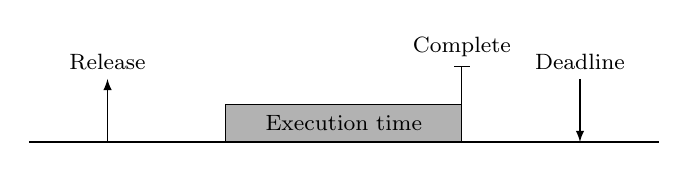
\begin{tikzpicture}[
  yscale = 0.8,
  normal/.style={fill=black!30},
  release/.style={-latex},
  complet/.style={-|},
  every text node part/.style={align=center}
]
%general params
\def\th{.6} %task height
\def\blockdim{(.4,.4)}
\def\arrowdim{(0,.5)}
\def\arrowdimB{(0,.4)}

%axes
\draw[thick, black] (0,0) -- (8, 0);

%L1
\draw[release] (1, 0) -- +(0,1) node[above] {{\footnotesize Release}};
\draw[normal]  (2.5, 0) rectangle +(3, \th) node[midway] {{\footnotesize Execution time}};
\draw[complet] (5.5, 0) -- +(0, 1.2) node[above] {{\footnotesize Complete}};
\draw[release] (7, 1) node[above] {{\footnotesize Deadline}} -- (7,0);

\end{tikzpicture}
}



\newcommand{\mrspSlideBis}{%
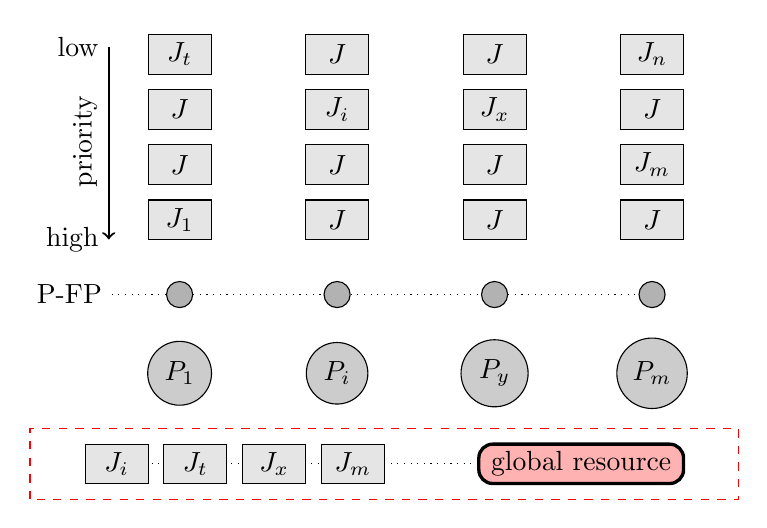
\begin{tikzpicture}[
  every text node part/.style={align=center},
  every circle node/.style={minimum width=.5ex},
  cpusty/.style={fill=gray!40,draw,circle,minimum width=1cm},
  task/.style={fill=black!10},
  sched/.style={fill=black!30,draw,circle,minimum width=1cm},
  ressty/.style={fill=red!30, draw, very thick, rounded corners=5pt}
]
%general params
\def\th{.5} %task height
\def\padding{.7}
\def\offset{.4}

% \partition{1};

  \node[cpusty] (P1) at (0+\offset,-1) {$P_1$};
  \node[sched]  (S1) at (0+\offset,0) {};

  \draw[task] (0.0,\padding*1) rectangle +(0.8, \th) node[midway,black]{$J_1$};
  \draw[task] (0.0,\padding*2) rectangle +(0.8, \th) node[midway,black]{$J$};
  \draw[task] (0.0,\padding*3) rectangle +(0.8, \th) node[midway,black]{$J$};
  \draw[task] (0.0,\padding*4) rectangle +(0.8, \th) node[midway,black]{$J_t$};

  \node[cpusty] (PI) at (2+\offset,-1) {$P_i$};
  \node[sched]  (SI) at (2+\offset,0) {};

  \draw[task] (2,\padding*1) rectangle +(0.8, \th) node[midway,black]{$J$};
  \draw[task] (2,\padding*2) rectangle +(0.8, \th) node[midway,black]{$J$};
  \draw[task] (2,\padding*3) rectangle +(0.8, \th) node[midway,black]{$J_i$};
  \draw[task] (2,\padding*4) rectangle +(0.8, \th) node[midway,black]{$J$};

  \node[cpusty] (PY) at (4.0+\offset,-1) {$P_y$};
  \node[sched]  (SY) at (4.0+\offset,0) {};

  \draw[task] (4,\padding*1) rectangle +(0.8, \th) node[midway,black]{$J$};
  \draw[task] (4,\padding*2) rectangle +(0.8, \th) node[midway,black]{$J$};
  \draw[task] (4,\padding*3) rectangle +(0.8, \th)  node[midway,black]{$J_x$};
  \draw[task] (4,\padding*4) rectangle +(0.8, \th) node[midway,black]{$J$};

  \node[cpusty] (PN) at (6.0+\offset,-1) {$P_m$};
  \node[sched]  (SN) at (6.0+\offset,0) {};

  \draw[task] (6,\padding*1) rectangle +(0.8, \th) node[midway,black]{$J$};
  \draw[task] (6,\padding*2) rectangle +(0.8, \th) node[midway,black]{$J_m$};
  \draw[task] (6,\padding*3) rectangle +(0.8, \th) node[midway,black]{$J$};
  \draw[task] (6,\padding*4) rectangle +(0.8, \th) node[midway,black]{$J_n$};
  
  \draw[dotted] (S1) -- (SI);
  \draw[dotted] (SI) -- (SY);
  \draw[dotted] (SY) -- (SN);

  \node (PFP) at (-1,0) {P-FP};
  \draw[dotted] (PFP) -- (S1);

  \draw[thick,->] (-.5,\padding*4.5) node[left,black]{low} node[rotate=90,left,xshift=-0.5cm,yshift=0.3cm]{priority} -- (-.5,\padding*1) node[left,black]{high};

  \begin{scope} [xshift=-0.8cm, yshift=-2.4cm]

  \draw[dashed, red] (-0.7,-0.2) rectangle (8.3,0.7);

  \draw[dotted] (0,0.25) -- +(5,0);
  \draw[task] (0,0) rectangle +(0.8, \th) node[midway,black]{$J_i$};
  \draw[task] (1,0) rectangle +(0.8, \th) node[midway,black]{$J_t$};
  \draw[task] (2,0) rectangle +(0.8, \th) node[midway,black]{$J_x$};
  \draw[task] (3,0) rectangle +(0.8, \th) node[midway,black]{$J_m$};

  \draw[ressty] (5,0) rectangle +(2.6,.5) node[midway]{global resource};

  % \node[inner sep=0pt] (arrow) at (8.5,1.2) {\includegraphics[width=.1\textwidth]{images/redArrow.png}};

  \end{scope}
 
\end{tikzpicture}
}

% \newcommand{\overheadsSuffered}[2]{%
% \begin{tikzpicture}[
%   xscale=#1,
%   yscale=#2,
%   every node/.append style={transform shape},
%   queuesty/.style={fill=white, very thick, font=\tiny},
%   srpsty/.style={fill=white, draw, circle, text width=.17cm, font=\tiny, very thick},
%   numsty/.style={text width=.1cm, font=\tiny},
%   arrow/.style={->},
%   littletext/.style={font=\sffamily\tiny,inner sep=0pt,outer sep=-2pt,fill=white},
%   ressty/.style={fill=red!30, draw, very thick, rounded corners=5pt},
%   emptytask/.style={rectangle, minimum width=.7cm,font=\footnotesize},
%   taskHolder/.style={fill=blue!90, draw, rectangle, minimum width=.7cm,font=\footnotesize},
%   taskWaiting/.style={fill=blue!70, draw, rectangle, minimum width=.7cm,font=\footnotesize,postaction={pattern=north east lines, very thin, pattern color=white}},
%   taskAccess/.style={fill=blue!30, draw, rectangle, minimum width=.7cm,font=\footnotesize},
%   taskNotAccess/.style={fill=white, draw, rectangle, minimum width=.7cm,font=\footnotesize}]

% \def\blockdim{(.7,.25)}

% \draw[arrow] (2.2,5.25) to[out=90,in=0] (2.35,6.6);

% \begin{scope}[xshift=2.2cm, yshift=5cm]
%   \coordinate (SRPnode) at (0,0);

%   \draw[dashed,purple] (-1.5,-0.78) -- (0.27,-0.78);

%   \node[taskNotAccess]  (T1)  at (-0.8,-0.50)  {};
%   \node[emptytask]      (TP1) at (-0.8,-0.75) {$\cdots$};
%   \node[taskWaiting]     (T2)  at (-0.8,-1.00)  {};
%   \node[emptytask]      (TP1) at (-0.8,-1.25) {$\cdots$};
%   \node[taskAccess]     (T3)  at (-0.8,-1.50)  {};
%   \node[emptytask]      (TP1) at (-0.8,-1.75) {$\cdots$};
%   \node[taskNotAccess]  (T4)  at (-0.8,-2.00)  {};
%   \node[emptytask]      (TP1) at (-0.8,-2.25) {$\cdots$};
%   \node[taskNotAccess]     (T5)  at (-0.8,-2.50)  {};

%   \draw[dashed, thin] ([shift={(-1.5,0)}]SRPnode) node[right,xshift=.1cm,littletext]{Partition$_2$} rectangle ([shift={(.3,-.15)}]T5.south-|SRPnode.east);

%   \node[srpsty] (SRP) at (SRPnode) {}; \node[font=\sffamily\tiny] at(SRPnode.west){SRP};
%   \draw[arrow] (T2.east) to[out=0,in=270] (SRP.south);

%   \draw[red] ([shift={(-.4,.17)}]T2) rectangle ([shift={(.25,-.05)}]T5.south-|T5.east);

%   \draw[arrow,red] (-0.35,-3.05) -- ([shift={(.1,-.05)}]T5.south-|T3.east);

% \end{scope}

\section{MrsP}

	\begin{frame}
	\frametitle{MrsP}
	\framesubtitle{Platform}	

		\begin{figure}
			\centering
			\scalebox{.8}{\mrspSlideBis}
			\caption{Partitioned Fixed-Priority scheduler on a platform with $m$ processors ($P_1$, \dots, $P_m$) and a global resource}
		\end{figure}

	\end{frame}

% \begin{frame}

% 	\frametitle{MrsP}
% 	\framesubtitle{Sharing resource in multiprocessor systems - 1}

% 	\begin{block}{Multiprocessor locking protocol}
% 		The serialization of access on parallel contention must guarantee:\\
% 		\begin{itemize}
% 			\item [(a)] bounded \alert{waiting time} to acquire the resource;
% 			\item [(b)] freedom from delaying repercussions for the jobs that don't require it (known as \alert{"independence preservation"}).
% 		\end{itemize}
% 	\end{block}

% 	\vspace{0.3cm}

% 	Furthermore \dots

% 	\vspace{0.3cm}

% 	\centerline{Unbounded waiting time $\rightarrow$ unbounded \alert{blocking time}}
	
% 	% An unbounded waiting time raises the \alert{blocking time} suffered by the jobs when a lower priority job will execute with an inherited ceiling priority equal or higher than its priority.\\

% \end{frame}

% \begin{frame}

% 	\frametitle{MrsP}
% 	\framesubtitle{Sharing resource in multiprocessor systems - 1}

% 	\begin{figure}
% 		\centering
% 		\scalebox{1}{\waitingtime}
% 	\end{figure}

% 	\begin{itemize}
% 		\item 2 processors and 3 tasks, $prio(J_i) > prio(J_y) \iff i > y$
% 		\item $J_1$ and $J_2$ share a global resource
% 		\item \textcolor{red}{(1)} $J_1$ remains preemptable
% 		\item \textcolor{red}{(2)} $J_1$ inhibits preemption
% 	\end{itemize}

% \end{frame}


% \begin{frame}

% 	\frametitle{MrsP}
% 	\framesubtitle{Sharing resource in multiprocessor systems - 2}

% 	\begin{block}{\emph{Suspension-based} or \emph{spin-based} protocol}
% 		A job, attempting to access a busy resource, will self-suspend ($J_2$) or will perform busy-wait ($J_3$)
% 	\end{block}

% 	\begin{figure}
% 		\centering
% 		\scalebox{0.9}{\SuspOrSpin}
% 	\end{figure}

% \end{frame}

\begin{frame}
	\frametitle{MrsP}
	\framesubtitle{Multiprocessor resource sharing Protocol - 1}

%\cite{Burns:2013:SCM:2547348.2547350}
%\cite{Baker:1991:SSR:113595.113601}

	Burns and Wellings design a multiprocessor extension of PCP/SRP with the aim of adapt a schedulability analysis to the protocol

	%in \emph{"A Schedulability Compatible Multiprocessor Resource Sharing Protocol"}

	\vspace{0.2cm}

	\begin{block}{Response Time Analysis incorporating PCP/SRP}
		The parameter \textcolor{red}{$e_j$} reflects the \textbf{contention} for the resource ($r$):

		\vspace{0.2cm}
		\centerline{$\textcolor{red}{e_j} = | map(G(r)) | \times \textcolor{blue}{c_j}$}
		\vspace{0.2cm}
		\centerline{$R_i = C_i + max \text{\{\textcolor{red}{$e_j$}},\hat{b}\} + \sum\limits_{\tau_j \in hp(i)} \ceil{\frac{R_i}{T_j}} C_j$}
		\vspace{0.2cm}
		\centerline{$C_i = WCET_i + \sum\limits_{r^j \in F(\tau_i)} n_i \text{\textcolor{red}{$e_j$}}$}

	\end{block}

\end{frame}

\begin{frame}
	\frametitle{MrsP}
	\framesubtitle{Multiprocessor resource sharing Protocol - 2}

	\centerline{\MrsP{1.1}{1.1}}

	\begingroup
 	  \fontsize{9pt}{8pt}\selectfont
	\begin{block}{Protocol's properties}
		\begin{itemize}
			\item It inherits the properties of PCP/SRP
			\item At most one job per processor requires the resource
			\item The length of the requests queue is at most $| map(G(r_j)) |$
			\item At most $e_j$ to gain the resource and to execute the critical section
		\end{itemize}
	\end{block}
	\endgroup


	% \begingroup
 	%   \fontsize{9pt}{8pt}\selectfont
	% 	\begin{enumerate}
	% 	\item access to global resources through local PCP/SRP;
	% 	\item \emph{spin at local ceiling} (remaining preemptable);
	% 	\item requests queued in a global FIFO;
	% 	\item assuming availability of a helping mechanism.
	% 	\end{enumerate}
	% \endgroup

\end{frame}

% \begin{frame}
% 	\frametitle{MrsP}
% 	\framesubtitle{Multiprocessor resource sharing Protocol - 3}	

% 	\begin{block}{Protocol's properties}
% 		\begin{itemize}
% 			\item it inherits the properties of PCP/SRP;
% 			\item at most one job per processor requires the resource;
% 			\item the length of the requests queue is at most $| map(G(r_j)) |$;
% 			\item a job requires at most $e_j$ to gain the resource and to execute the critical section.
% 		\end{itemize}
% 	\end{block}

% \end{frame}

% \begin{frame}
% 	\frametitle{MrsP}
% 	\framesubtitle{Runtime example}

% 	\centerline{\MrsPProtocols}

% 	\begin{itemize}
% 	\item $t_1$: $J_1$'s priority is raised: it gains access to $r$
% 	\item $t_2$: $J_3$'s priority is raised: it starts spinning
% 	\item $t_3$: $J_2$ is released and $J_3$ "helps" $J_1$
% 	\end{itemize}
% \end{frame}